\section{INTRODUCTION}

\bulletpoints{
    \item Topic Sentence: This paragraph should introduce the problem/challenge. It should briefly discuss the FK model and how it is solved.
    \item Give a brief overview of CTCRs and the Cosserat Rod Model
    \item The use of a numerical approach should be mentioned to explain how the interactions between the tubes are modelled
    \item Reference Rucker's paper and mention that a BVP is used to solve the model.
    \item Mention that it is the gold-standard and briefly discuss the high computational cost associated with the BVP
}

\commentblock{
Concentric tube continuum robots (CTCRs), as shown in Fig. ~\ref{fig:ctcr}, consist of multiple concentric, precurved, super-elastic tubes that can be rotated and translated relative to one another \cite{WebsterOkamuraCowan_IROS_2006, SearsDupont_IROS_2006}.
Due to the complex elastic interactions between the tubes, numerical tools are often needed to capture the highly non-linear behaviour of robots with more than two tubes \cite{DupontLockItkowitzButler_TRO_2010}.
Rucker et al. introduced in \cite{RuckerJonesWebster_TRO_2010} a highly-accurate physics model based on Cosserat rod theory, formulating the robot's kinematics as a boundary value problem (BVP) with unknown initial conditions.
Although this model is the gold-standard for CTCR modeling, there is a high computational cost associated with solving its BVP.

\begin{figure}
    %\fbox{
    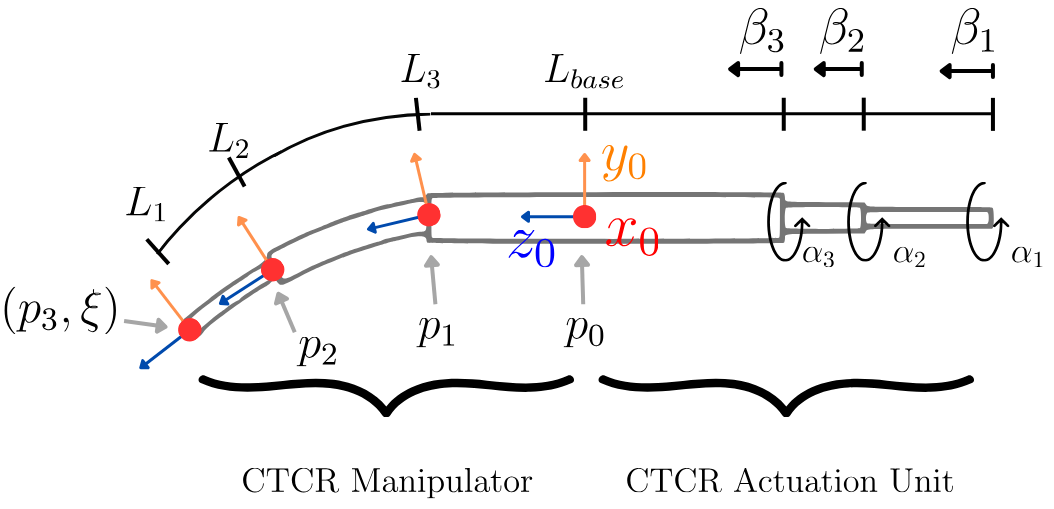
\includegraphics[width=\columnwidth]{Figures/CTCR.png}
    %}
    \caption{
    Diagram of an annotated CTCR consisting of three precurved tubes. Please note that the innermost, middle, and outermost tubes are referenced with the indices 1, 2, and 3 respectively.
    }
    \label{fig:ctcr}
\end{figure}
}

\bulletpoints{
    \item Topic Sentence: To justify the problem mentioned in the previous paragraph, this paragraph should introduce to the reader the literature on Cosserat Rod optimizations. The goal is to convince the reader that although there has been a lot of work in this area, there has been no definite, universal approach to optimize the problem.
    \item Provide a brief overview of the various efforts that have been undertaken to optimize the problem
    \item Categorize these efforts into the universal-approaches (architecture and hardware agnostic) vs system-specific approaches
    \item Discuss the level of optimization that each approach achieved and compare them.
    \item Argue that there remains a need for an optimization approach that achieves real-time control while being universal.
}

\commentblock{
Efforts to optimize the computational cost of solving the Cosserat rod model have been extensive, yet no universal approach has emerged.
While some studies offer broad, architecture-agnostic improvements, they often fall short of real-time control, achieving execution times of $40$ ms and $57$ ms respectively \cite{RuckerWebster_ICRA_2011, OrekhovSimaan_IROS_2020}.
Other optimizations achieve real-time performance but are limited by specific robot architectures \cite{TillBrysonChungOrekhovRucker_ICRA_2015} or actuation systems \cite{XuPatel_EMBC_2012}.
Despite these advancements, there remains a critical need for an optimization strategy that not only achieves real-time control but is also universally applicable, balancing generalized performance with real-time execution across various systems.
}

\bulletpoints{
    \item Topic Sentence: In this paragraph, I want to explain what our contribution to the field is. I want to discuss how we attempted to solve the problem stated above and what our final solution is. Lastly, I want to discuss our results and why they are significant (at least to me).
    \item Explain the framework/approach used to solve this problem.
    \item Discuss why the optimization strategy used ensures universality.
    \item Discuss the runtime improvement achieved and why it is significant.
    \item Discuss the potential proxy to elastic stability and why it is significant.
}

\commentblock{
This paper presents a comprehensive investigation of the numerical tools used in the computation of the static forward kinematics (FK) of CTCRs.
We introduce a variety of numerical optimization techniques that result in significant runtime reductions with no compromise in accuracy, enabling real-time performance while maintaining universal applicability across model implementations.
Additionally, we demonstrate a potential numerical proxy for assessing the robot's elastic stability which opens up new possibilities for stable path planning in CTCR systems.
}

\subsection{State of the Art}

\bulletpoints{
    \item Topic Sentence: A brief and quick introduction to the state of the art. This section should explain how the BVP is currently solved (classical RK4 with Newton-Raphson solver) and why (no need to perserve group structure, ease of use in Matlab, etc).
    \item Discuss the shooting method and why it is used to solve the BVP
    \item Briefly explain why there is no need to perserve rotation group structure.
    \item Discuss the integrator used and why it is used
    \item Discuss the solver used and why it is used
}

\commentblock{
Current state-of-the-art approaches for solving the BVP primarily use explicit Runge-Kutta methods combined with the Newton-Raphson nonlinear solver \cite{RuckerJonesWebster_TRO_2010, RuckerWebster_ICRA_2011, Gilbert_Springer_2016, Burgner-Kahrs_TRO_2015}.
This combination is favored due to its robustness and ease of use, particularly in environments like \textsc{MATLAB} \cite{RuckerJonesWebster_TRO_2010, RuckerWebster_ICRA_2011, TillBrysonChungOrekhovRucker_ICRA_2015}.
Although it was initially believed that specialized integrators were needed to preserve rotation group structure \cite{DupontLockItkowitzButler_TRO_2010}, the error from standard explicit integrators has been shown to be negligible compared to the model's inherent kinematic error \cite{Gilbert_Springer_2016, DieciRussellVanVkeck_SIAM_1994}.
The shooting method is commonly employed in this framework, effectively guiding the solution towards convergence.
}